\section{Flowchart}
A flowchart is a type of diagram that represents an algorithm, work flow or process, showing the steps as boxes of various kinds, and their order by connecting them with arrows
and the flowchart \ref{fig:FD1} of Rebar Addon showing the flow of control and Data in the software.

\begin{figure}
	\centering \includegraphics[width=\linewidth]{images/RebaraddonDFD.png}
	\caption{Flowchart of Rebar Addon}
	\label{fig:FD1}
\end{figure}

\subsection{Detailed Description}

The basic implementation of this project is almost done in form of prototype. There is need to modify the structure of the project. We have to divide the task into there parts:

\begin{enumerate}
	\item \textbf{Front end}
	It will deal with how the Rebar Addon will look to the user like in form of toolbars, menus etc. This part will include two parts:
	\begin{enumerate}
		\item \textbf{Rebar Addon toolbar/menus}
		It contains a list of different rebars.
		\item \textbf{Dialog box}
		A number of different inputs widgets present in the dialog box according user's selected rebar.
	\end{enumerate}
	
	\item \textbf{Back End}
	On backend, a top layer is created over FreeCAD rebar object which holds rebars properties (likes side cover, left cover, orientation and bent angle etc.) and then a rebar profile is created from these properties. This profile is now pass to Rebar object which will create rebar.  
	
\end{enumerate}


\section{Dependency Graph}
A Dependency Graph is a graphical representation of the which module is dependent on which other modules. A Dependency Graph is often used as a preliminary step to creating an overview of the system. Dependency Graph also gives overview of how good is the design of the system.
FreeCAD being were huge software it would be difficult to make the dependency graph of whole software. So, here is  Dependency Graph of Rebar addon is as following-:
\begin{enumerate}
\item \textbf{Caller graph of FreeCAD Rebar object:} Figure \ref{fig:comment1} shows the modules that use rebar object.
\item \textbf{Caller graph of StraightRebar.\_StraightRebarTaskPanel.clicked:} Figure \ref{fig:comment} shows the modules that use the module StraightRebar.\_StraightRebarTaskPanel.clicked.
\item \textbf{Caller graph of StraightRebar.\_StraightRebarTaskPanel.accept:} Figure \ref{fig:dependency} show the modules that uses the module StraightRebar.\_StraightRebarTaskPanel.accept.
\item \textbf{Caller graph of Rebar Distribution:} Figure \ref{fig:dependencyy} show the modules that uses the module Rebar Distribution.
\end{enumerate}

\begin{figure}
	\centering
	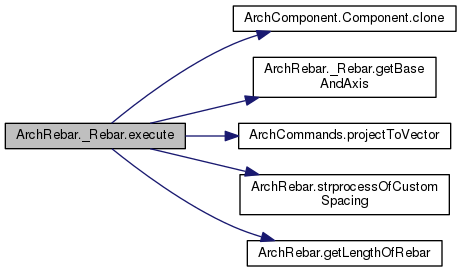
\includegraphics[scale=.8]{images/rebarobject.png}
	\caption{Dependency graph of Rebar object}
	\label{fig:comment1}
\end{figure}

\begin{figure}
\centering
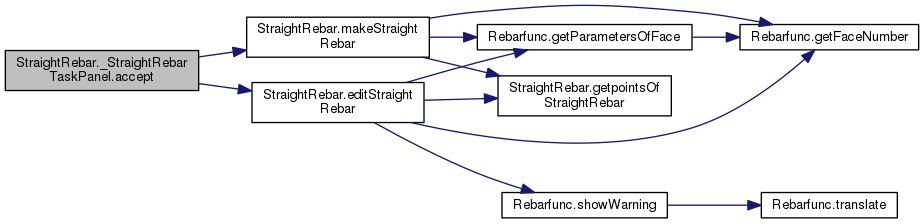
\includegraphics[width=1\linewidth]{images/taskpanelaccept.png}
\caption{Caller graph of StraightRebar.\_StraightRebarTaskPanel.clicked}
\label{fig:comment}
\end{figure}
\begin{figure}
\centering
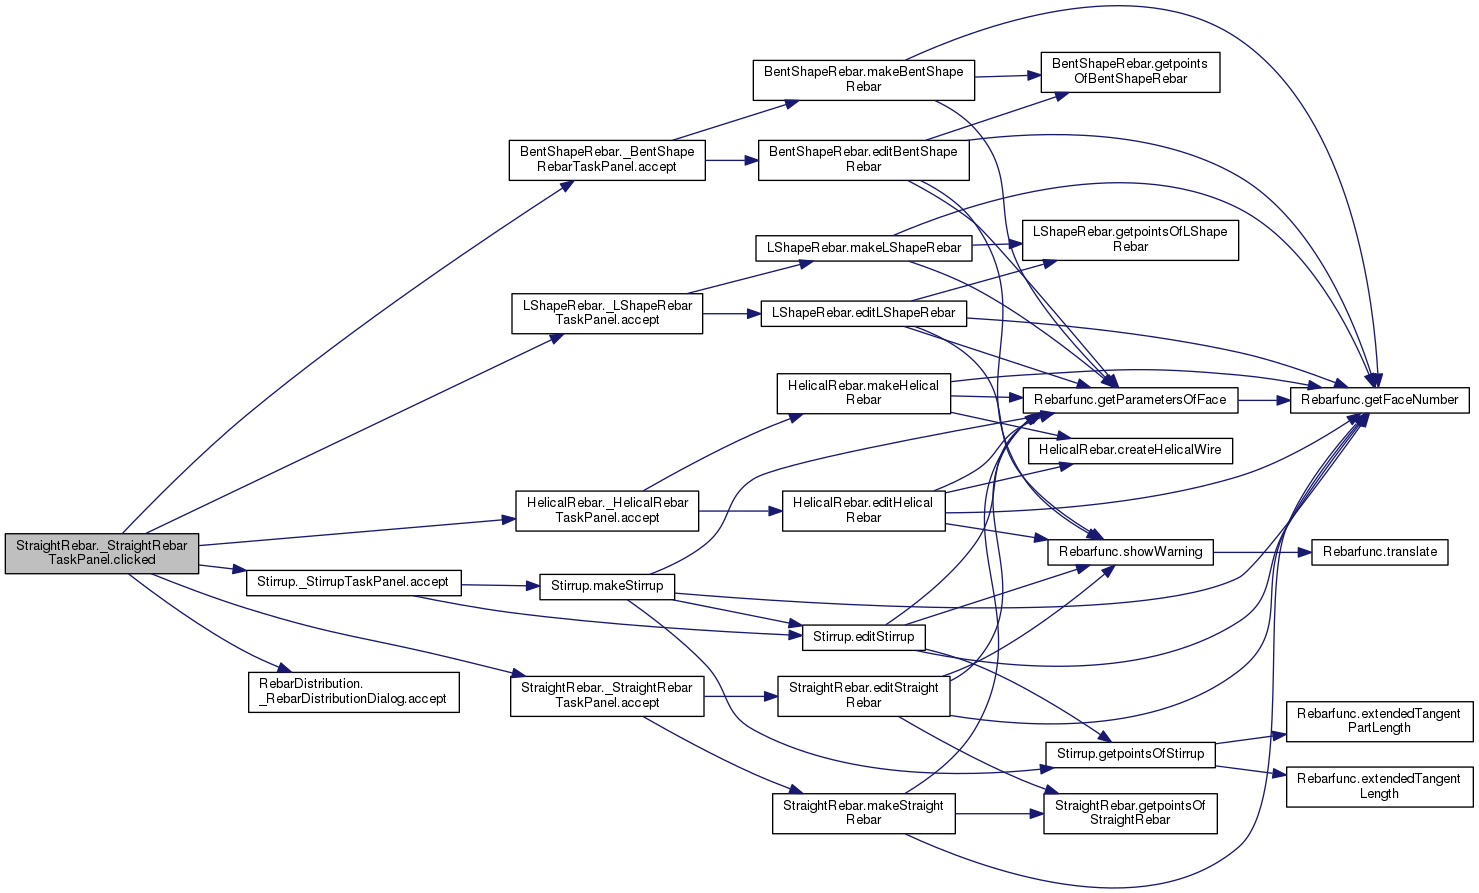
\includegraphics[width=1\linewidth,height=1\columnwidth]{images/taskpaneldetail.png}
\caption{Caller graph of StraightRebar.\_StraightRebarTaskPanel.accept}
\label{fig:dependency}
\end{figure}


\begin{figure}
\centering
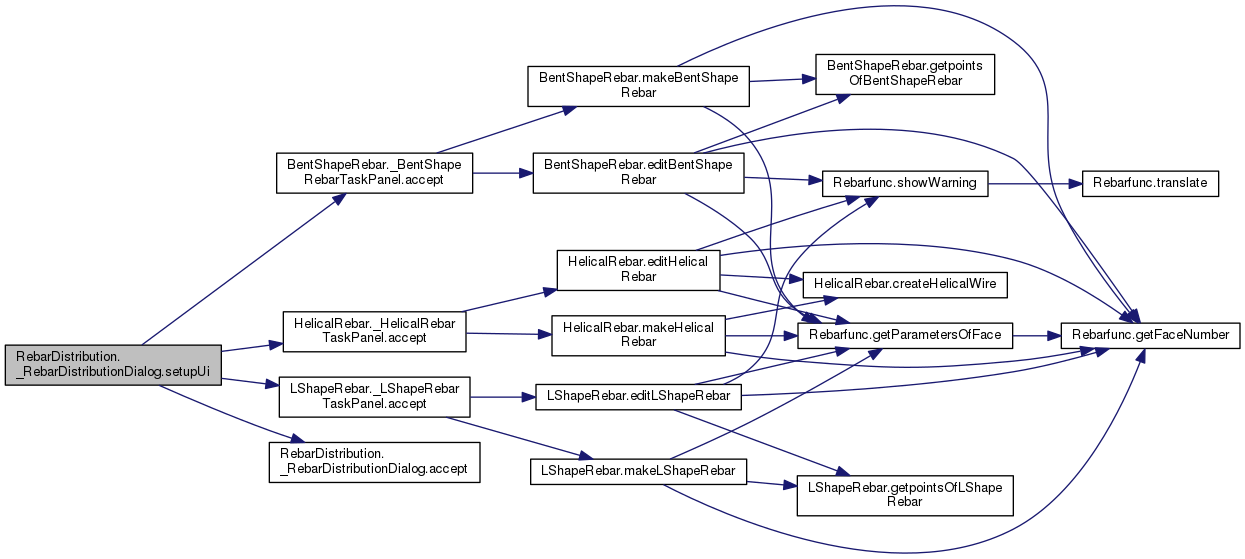
\includegraphics[width=1\linewidth,height=1\columnwidth]{images/rebardistribution.png}
\caption{Caller graph of RebarDistribution}
\label{fig:dependencyy}
\end{figure}


\section{Class Diagrams}
Class Diagrams describe the static structure of the system. Following classes diagram represent the relationship between different classes in FreeCAD and Rebar Addon:
\begin{enumerate}
	\item Figure \ref{fig:collaborative1} shows the class diagram of the ArchComponent.Component class which is the basse class of ArchRebar.\_Rebar i.e ParameterCheckbox, ParameterVector,ParmeterSpinbox, ParameterComboBox,ParameterSlider, ParameterText.

	\item Figure \ref{fig:collaborative} shows the class diagram of the StraightRebar.\_StraightRebarTaskPanel class which is the main class for whole the Straight rebar dialog box.
	
	\item Figure \ref{fig:classAnnotation__coll__graph}  shows the class diagram of the RebarDistribution.\_RebarDistributionDialog class which is the main class on rebar distribution dialog box.

	\item Figure \ref{fig:classAnnotation__coll__graphh}  shows the class diagram of the QtGui::QDialog which is the base class of PipUpImage.PopUpImage.
\end{enumerate}

\begin{figure}
    \centering
    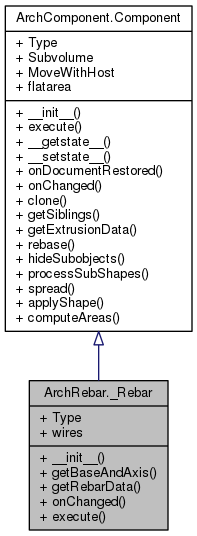
\includegraphics[scale=.85]{images/archRebar.png}
    \caption{Class Diagram for ArchRebar.\_Rebar}
    \label{fig:collaborative1}
\end{figure}

\begin{figure}
    \centering
    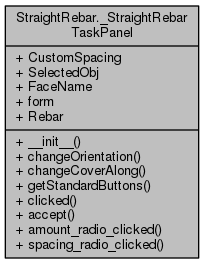
\includegraphics[scale=.85]{images/straightclass.png}
    \caption{Class Diagram for StraightRebar.\_StraightRebarTaskPanel}
    \label{fig:collaborative}
\end{figure}

\begin{figure}
\centering
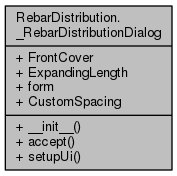
\includegraphics[scale=.85]{images/rebarDistributionclass.png}
\caption{Class Diagram for RebarDistribution.\_RebarDistributionDialog}
\label{fig:classAnnotation__coll__graph}
\end{figure}

\begin{figure}
\centering
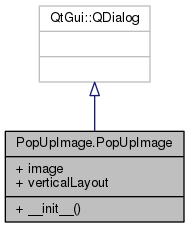
\includegraphics[scale=.85]{images/popupimage.png}
\caption{Class Diagram for PipUpImage.PopUpImage}
\label{fig:classAnnotation__coll__graphh}
\end{figure}
